\section{Implementation}
In diesem Kapitel beschäftigen wir uns mit der Implementation und mit dem Aufbau von Grafana, sodass wir \gls{Cyberangriff} nach dem \gls{mitre} Matrix erkennen können. Wir gestalten unser Arbeitslabor mit \gls{container} und \glsfirst{vm}, wie in dem folgenden Diagramm:

\begin{figure}[H]
   \centering
   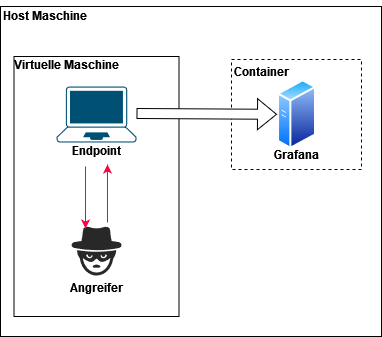
\includegraphics[width=0.8\textwidth]{assets/Arbeitslabor.drawio.png}
   \caption{Aufbau unseres Arbeitslabors \\Quelle: Eigene Quelle}
   \centering
\end{figure}

Von unserem Aufbau zielen wir, die Aufnahmen und Anpassung der Logdateien für Grafana, die Musterkerennung für die ausgewählten \glsplural{Cyberangriff} und schließlich die Warnmeldung für die Endnutzer, sodass sie sich für entsprechende Sicherheitsmßnahmen entscheiden können. 

\newpage
Der gewünschte Ablauf ist in dem folgenden Diagramm dargestellt:

\begin{figure}[H]
   \centering
   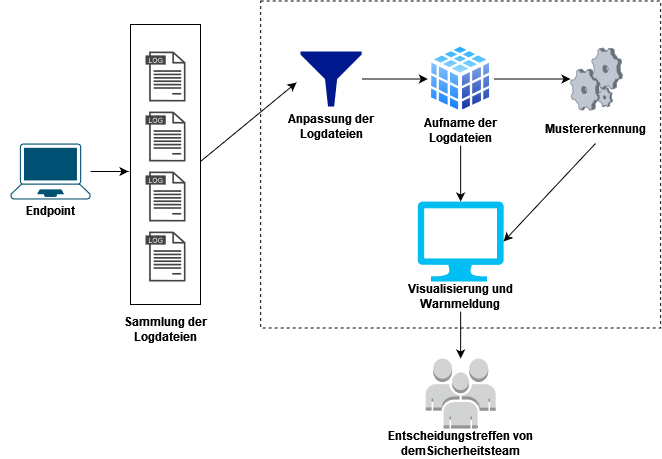
\includegraphics[width=1\textwidth]{assets/Ablauf_grafana.drawio.png}
   \caption{Erwarteter Ablauf von der Datensammlung bis zur Warnmeldung von \glsplural{Cyberangriff} \\Quelle: Eigene Quelle}
   \centering
\end{figure}

\subsection{Angriffserkennung anhand der Mitre ATT\&CK Matrix\textregistered}
Es gibt verschiedene Methode und Framework zur Vermeidung, Erkennung, und Unterbrechung von \glsplural{Cyberangriff}. \glsfirst{owasp}, \glsfirst{CKC} und \gls{mitre} Matrix sind einige Bespiele von denen, die \gls{SOC}-Teams verwenden, um Sicherheit von Systemen und/oder Netzwerken zu gewährleisten. Da die Richtlinien und Fokus von diesen Frameworks sich unterscheiden können und deswegen anderen Aufbau von unserer Struktur verlangen wurden, entschieden wir uns für die Anwendung von der \gls{mitre} Matrix für die Erkennung der \glsplural{Cyberangriff} besonders, weil dieser Framework auch an Splunk integriert ist.

Die \gls{mitre} Matrix hat folgende Hauptnutzung \citep{Mitre_Started}:

{\setstretch{1.5}
\begin{itemize}[noitemsep]
   \item Erkennung und Analyse von Angriffstechnik
   \item	strukturierte Datensammlung über Bedrohungen
   \item	Emulieren von \glsplural{Cyberangriff} für die Anwendung an Angriffsübungen
   \item	Systemhärtung und Verbesserung der Verteidigungsmaßnahmen
\end{itemize}
}

Die Matrix bietet eine umfangreiche Verwendung für Unternehmen und für \gls{SOC}-Team an, um ihre wertvollen Ressource schützen und ihre Fachkenntnisse über \gls{Cybersicherheit} zu erweitern \citep{Hazel_howtousemitre}. Hier konzentrieren wir uns auf die Entwicklung und auf die Implementierung einer Methode für die automatische Erkennung und Analyse von Angriffstechnique in Grafana.

Die \gls{mitre} Framework besteht aus 14 Taktik. Zu jedem Taktik gehören Technique, die ihrerseits in Subtechniques aufgeteilt sind. Jede Subtechnique wird mit Beispielen, Härtungsmaßnahmen und Erkennungsregeln dargestellt. Die nächste Abbildung zeigt, wie diese Struktur aufgebaut ist: 

\begin{figure}[H]
   \centering
   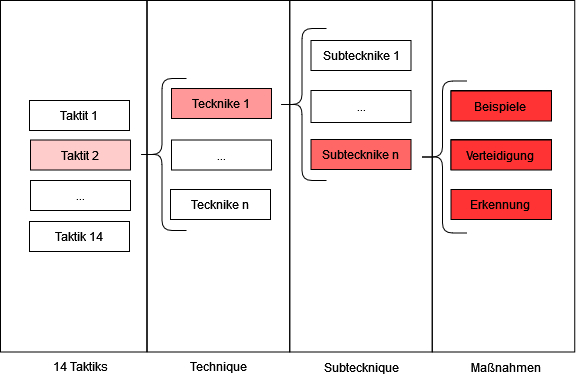
\includegraphics[width=0.8\textwidth]{assets/Mitre_structure.drawio.png}
   \caption{Struktur der Mitre Matrix \\Quelle: Eigene Quelle und \citep{Mitre_Started}}
   \centering
\end{figure}

{\setstretch{1.5}
Die 14 Tactics sind folgende:
\begin{itemize}[noitemsep]
   \item Informationssammlung für zukünftige Angriffe 
   \item	Entwicklung von Ressource von Angreifer
   \item Erster Zugang zum Opfersysteme 
   \item Ausführung von bösartigen Coden
   \item Beharrlichkeit von System
   \item	Privilegienausweitung
   \item Vermeidung von Verteidigungssysteme
   \item Zugang zu Anmeldedaten
   \item Umgebungserkennung
   \item Seitliche Bewegung zu anderem Systemen innerhalb des Angriffsziels
   \item interne Informationssammlung
   \item Steuerung und Kontrolle (C2 - Command and Control im Original)
   \item Datenextrahierung 
   \item	Auswirkung auf die Integrität
\end{itemize}
}

\subsection{Auswahl des Angriffes}
In dieser Arbeit beschäftigen wir uns mit dem Tactic \quotes{Zugang zu Anmeldedaten} und deren Technique \gls{bruteforce}. Diese Technique ist in vier Subtechnique aufteilt:

{\setstretch{1.5}
\begin{itemize}[noitemsep]
   \item Erraten von Anmeldedaten 
   \item	Entschlüsselung von \glsplural{hash}
   \item \textit{\gls{stuffing}}
   \item \textit{\gls{spraying}}
\end{itemize}
}

Da unser Ziel hier ist Grafana, zu benutzen, um Angriffe zu erkennen, entschieden wir uns für einen einfachen reproduzierbaren Angriff, die weniger Ressource verlangt. In diesem Fall, lässt sich \gls{bruteforce} einwandfrei mit zwei \glsplural{vm} darstellen. Für diesen Angriff benutzen wir die Subtechnique \quotes{Erraten von Anmeldedaten und \textit{\gls{stuffing}}}, da sie ähnliche Erkennungmethode haben. Hier schließen wir auch die anderen Maßnahmen aus.

Die nächste Abbildung zeigt den Umfang unseres Implementationsversuchs:
\begin{figure}[H]
   \centering
   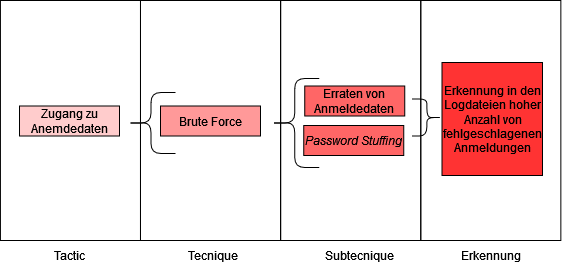
\includegraphics[width=0.8\textwidth]{assets/T1110.drawio.png}
   \caption{Analysestruktur für diese Arbeit \glsplural{Cyberangriff} \\Quelle: Eigene Quelle und \citep{Mitre_t1110}}
   \centering
\end{figure}

\subsection{Installation und Erstellung von Logdateien}
In diesem Abschnitt fokussieren wir uns auf folgenden Punkten:

\begin{enumerate}[noitemsep]
   \item	Einrichtung der \glsplural{vm} für Opfersystem und Angreifen
   \item	Angriffsssimulation für die für die Generierung von Logdateien
   \item Installation und Einrichtung von Grafana Loki und Promtail mit \gls{container}
\end{enumerate}

Die Installation und Anwendung können entweder mit dem \gls{GUI} oder mit der Kommandozeilen durchgeführt werden. In dieser Arbeit benutzen wir die Kommandozeile. 

\subsubsection{Einrichtung der \glsplural{vm} für Opfersystem und Angreifen}
Die beiden \glsplural{vm} sind \quotes{\gls{kali} vorgebaute \glsfirst{vm}} und \quotes{\gls{ubuntu} Server 22.04.2} in ihren standardmäßigen Einstellungen. Beiden Maschinen lassen sich aus der jeweiligen Schritte Dokumentation einwandfrei installieren \citep{kali_vm} und \citep{Ubuntu_server}.

Für das Opfersystem entschieden wir uns für das Passwort \quotes{qwertz}. Laut einer Umfrage gehört dieses Passwort zu den zehn meisten verwendeten Passwort in Deutschland \citep{silicon_passwort}.  

Für die Durchführung von \gls{spraying} erstellen wir folgende Benutzer und Passwörterkombinationen:
{\setstretch{1.0}
\begin{verbatim}
   admin:123456
   user1:passwort
   user2:abc123
   user3:qwertyuiop
\end{verbatim}
}

\subsubsection{Angrifsssimulation für die für die Generierung von Logdateien}
Für den Angriff verwenden wir folgenden Tools:
\begin{itemize}[noitemsep]
   \item	\glsfirst{ssh}
   \item \gls{hydra}
\end{itemize}

In diesem Szenario schickt \gls{hydra} gleichzeitig mehrere Authentifizierungsversuche zum Opfersystem, um eine \gls{ssh} Verbindung mit dem Opfersystem zu erstellen. Das Tool verwendet ein sogenanntes Wörterbuch mit verschiedenen Einträgen, die als Passwörter dienen. Für unseren Test benutzen wir die bekannten Datei \gls{rockyou} Datei. 

\newpage
Die nächste Abbildung zeigt, wie \gls{stuffing} abläuft:

\begin{figure}[H]
   \centering
   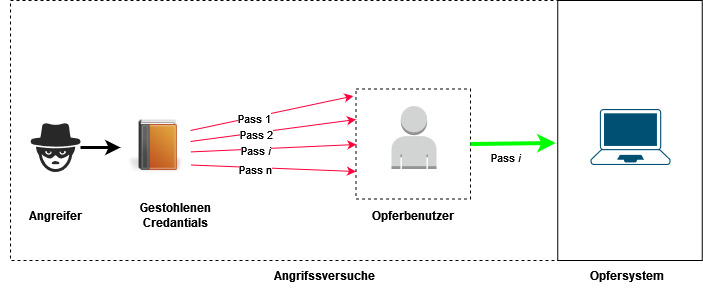
\includegraphics[width=0.7\textwidth]{assets/Stuffing.jpg}
   \caption{\textit{\gls{stuffing}}\\Quelle: Eigene Quelle und \citep{Nguyen_stuffing}}
   \centering
\end{figure}

Das folgende Kommando wurde gegen das Angreifersystem für \gls{stuffing} ausgeführt \citep{kali_hydra}:
{\setstretch{1.0}
\begin{spverbatim}
   hydra -l test -P rockyou.txt [Adresse von Opfersystem] ssh -V -t 4

   # Erklärung
   -l: Spefizikation der Benutzername, den wir Angreifen
   -P: Auswahl der Datei mit bekannten Passwörter
   ssh: Auswahl der Anwendung, die wir angreifen wollen
   -V: Ausgabe ausführlicher Information über die Durchführungen, wie Versuche, Fehlermeldungen und Erfolge
   -t 4: Anzahl von gleichzeitigen Verbindungen
\end{spverbatim}
}

Das folgende Bild zeigt ein Teil der Ausgabe von \gls{hydra} bei der Ausführung von \gls{stuffing}:
\begin{figure}[H]
   \centering
   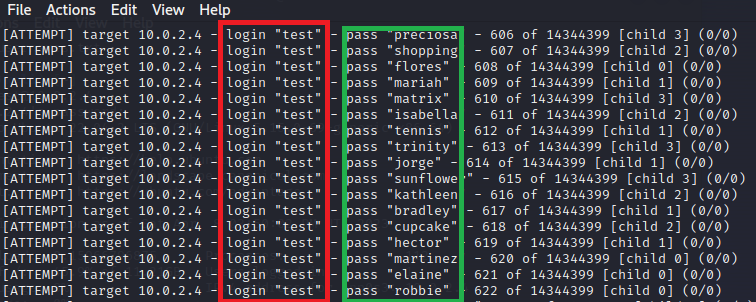
\includegraphics[width=0.7\textwidth]{assets/stuffing_kali.png}
   \caption{\textit{\gls{stuffing}}\\Quelle: Eigene Quelle und \citep{Nguyen_stuffing}}
   \centering
\end{figure}

Unser nächster Angriff, \gls{spraying}, sieht wie folgende aus:
\begin{figure}[H]
   \centering
   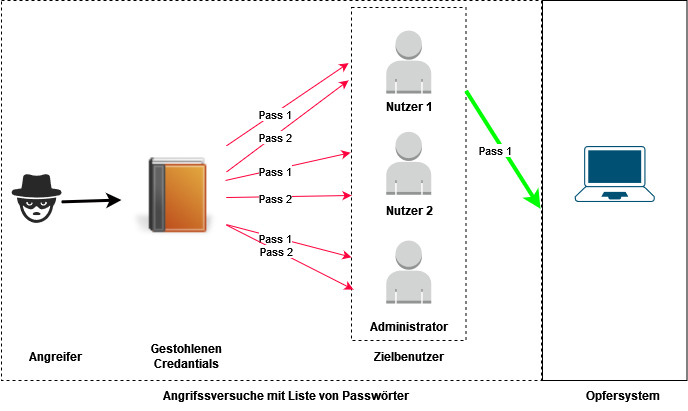
\includegraphics[width=0.7\textwidth]{assets/Spraying.jpg}
   \caption{\textit{\gls{spraying}}\\Quelle: Eigene Quelle und \citep{Swathi_spraxy}}
   \centering
\end{figure}

Für diesen Angriff benutzen wir dasselbe Kommando wie vorher, mit einem \quotes{-L} (großen \quotes{L}) anstelle von \quotes{-l} (kleinen \quotes{L}). \quotes{-L} deutet darauf hin, dass wir eine Textdatei mit verschiedenen Benutzernamen verwenden 

Der folgende Screenshot zeigt die Ausführung von \gls{spraying}:
\begin{figure}[H]
   \centering
   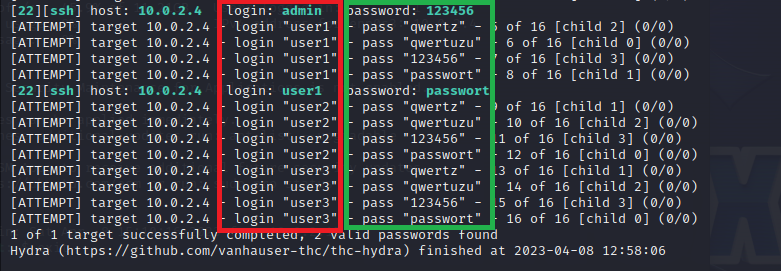
\includegraphics[width=0.8\textwidth]{assets/Spraying_Kali.png}
   \caption{Ausführung \textit{\gls{spraying}} in Kali Linux \\Quelle: Eigene Quelle}
   \centering
\end{figure}

\subsubsection{Installation und Einrichtung von Grafana Loki und Promtail mit \gls{container}}
Die offizielle Dokumentation von Grafana war nicht immer über die Ausführung eindeutig, deshalb benutzten wir auch fremde Quellen verwendet, um die Einstellungen an unsere Umgebung anzupassen \citep{Polinowski_PGL}. Unter befindet es sich die von Grafana zur Verfügung gestellte Konfigurationsdateien und Installationsverfahren \citep{GrafanaLoki_run}. 

{\setstretch{1.0}
\begin{spverbatim}
wget https://raw.githubusercontent.com/grafana/loki/v2.8.0/cmd/loki
/loki-local-config.yaml -O loki-config.yaml (die Datei wurde angepasst)

wget https://raw.githubusercontent.com/grafana/loki/v2.8.0/clients/
cmd/promtail/promtail-docker-config.yaml -O promtail-config.yaml 
(die Datei wurde angepasst)

docker-compose -f docker-compose.yaml up 
\end{spverbatim}
}
%docker run -d --name=grafana -p 3000:3000 grafana/grafana-enterprise
%docker run --name loki -d -v $(pwd):/mnt/config -p 3100:3100 grafana/loki:2.8.0 -config.file=/mnt/config/loki-config.yaml

%docker run --name promtail -d -v $(pwd):/mnt/config -v /var/log:/var/log --link loki grafana/promtail:2.8.0 -config.file=/mnt/config/promtail-config.yaml

Im Anhang befinden sich die originalle und die angepassten Dateien.

\textcolor{red}{\textbf{Anhänge hinzufügen}}te

Die obigen Kommandos haben folgende Bedeutungen:
\begin{enumerate}[noitemsep]
   %\item Ausführung von Grafana und Nutzung des Nutzung des lokalen und externen \glsplural{port} 3000
   \item Herunterladen der Konfigurationsdatei von Loki
   %\item Ausführung der Loki \gls{container}, Nutzung des lokalen und externen \glsplural{port} 3100 für die Netzwerkverbindung und Verwendung der heruntergeladenen Konfigurationsdatei
   \item Herunterladen der Konfigurationsdatei von Promptail
   %\item Ausführung der Promptail \gls{container}, Verbindung zwischen diesen und den Loki \gls{container} und Verwendung der heruntergeladenen Konfigurationsdatei
   \item Ausführung von den \glsplural{container}, indem beiden Konfigurationsdateien in einer eingepackt und angepasst wurden und schliesslich von der \gls{container}-Anwendung gelesen werden
\end{enumerate}

Für spezifische Versionen oder andere weitere Einstellungen bietet die Dokumentation umfangreiche Möglichkeiten an \citep{GrafanaLoki_run}.

Für diesen ersten Test, wurden die Logdatei des Opfersystems manuell zu dem \gls{container} übertragen.

\newpage
\thispagestyle{lscape}
\begin{landscape}
   Nach der Ausführung des Kommandos ist die Anwendung schon benutzbar, wie in dem folgenden Screenshot:
   \begin{center}
      \begin{figure}[H]
         \centering
         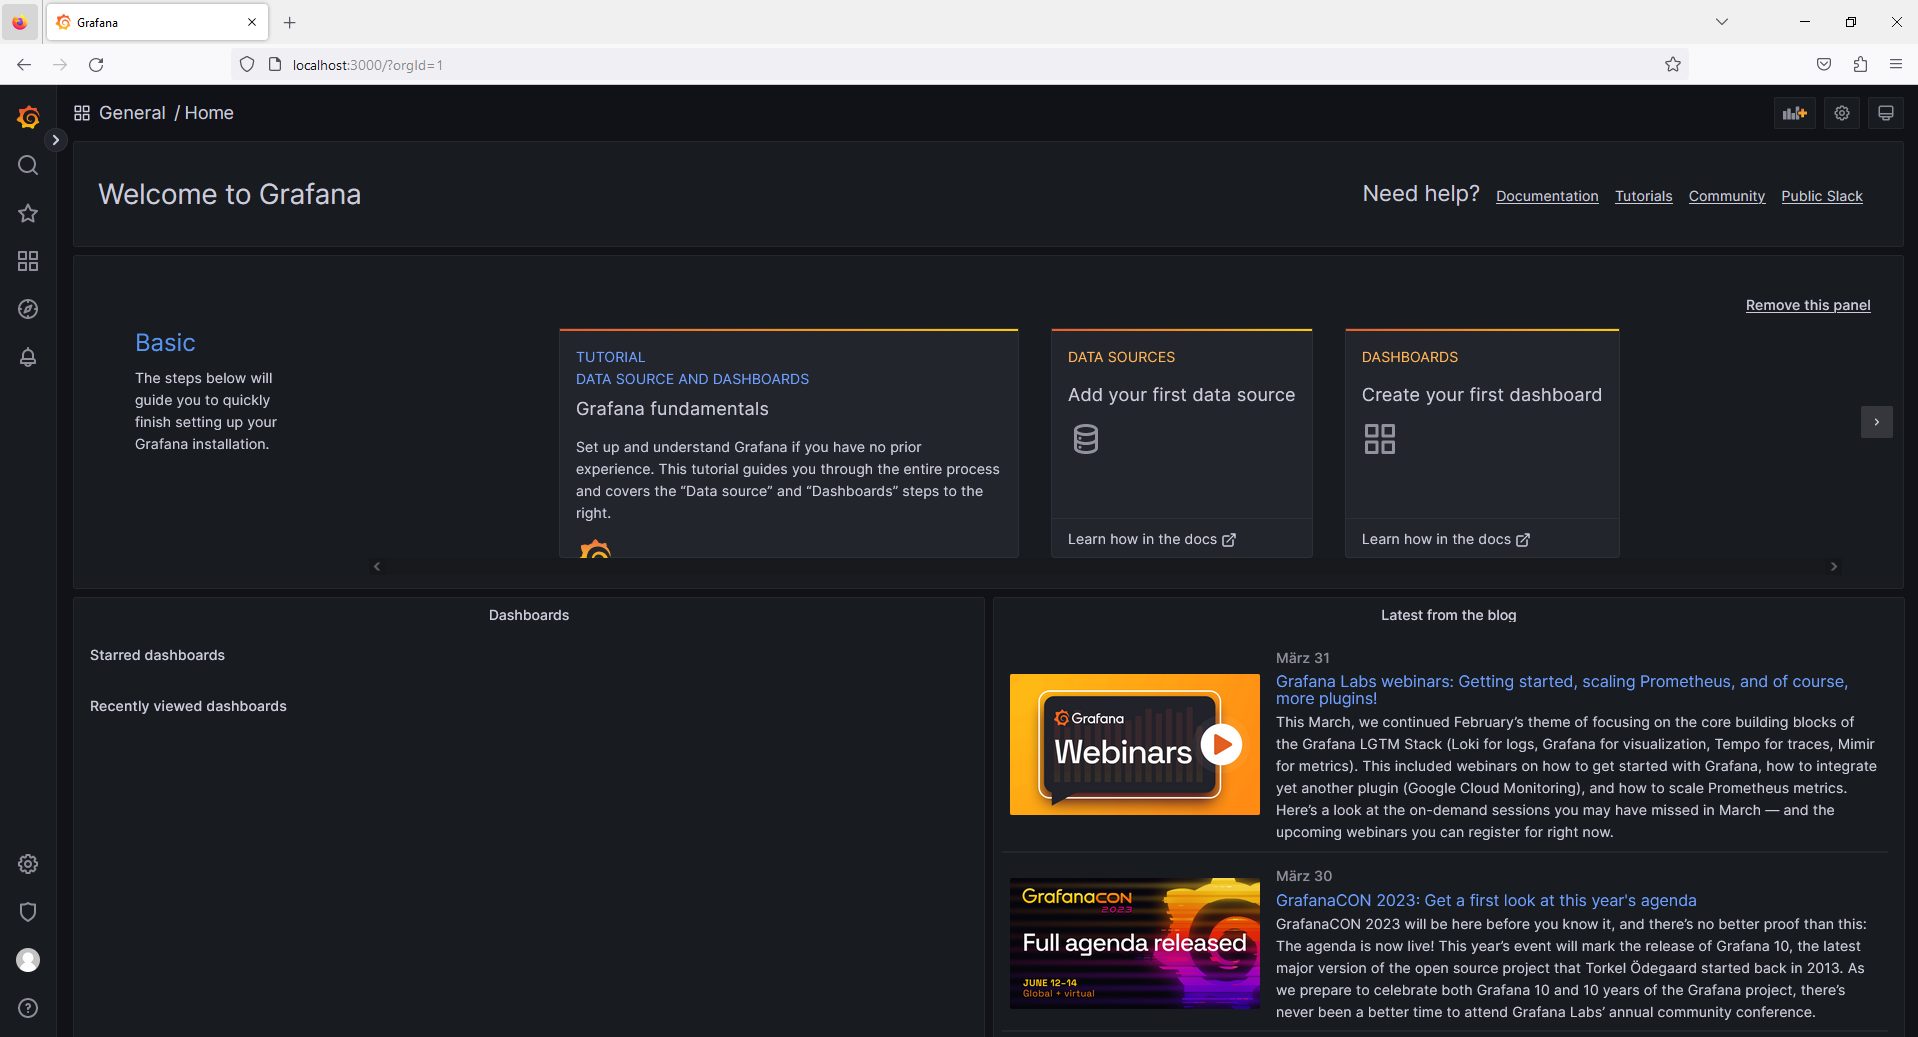
\includegraphics[width=1.3\textwidth]{assets/Installation_Grafana.png}.
         \caption{Screenshot der Willkommensseite von Grafana Loki\\Quelle: Eigene Quelle und \citep{Grafana_Logs}}
         \centering
      \end{figure}
   \end{center}
\end{landscape}

\subsection{Aufbau der Erkennungsregel für den ausgewählten Angriff}
Der \gls{bruteforce} lässt sich durch die Anzahl des fehlgeschlagen Anmeldungsversuchs erkennen \citep{Selvaganesh_SplunkBruteForce}. Wir bearbeiten eine Situation, in der es keine Gegenmaßnahmen, wie Kontosperre nach \textit{n} beliebigen Versuchen oder \gls{mfa}, implementiert sind. Das folgende Aktivitätsdiagramm stellt einen allgemeinen Ablauf eines Anmeldungsverfahrens dar:

\begin{figure}[H]
   \centering
   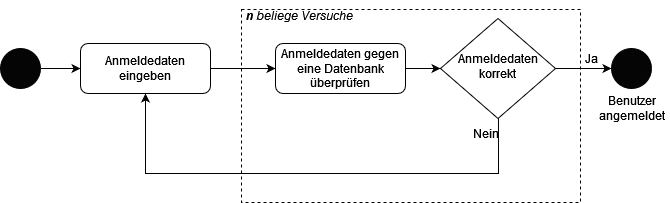
\includegraphics[width=0.8\textwidth]{assets/Anmeldeverfahren.drawio.png}
   \caption{Allgemeiner Ablauf eines Anmeldungsverfahrens \\Quelle: Eigene Quelle und \citep{Selvaganesh_SplunkBruteForce}}
   \centering
\end{figure}

Eine Erkennungsregel würde der unteren Logik folgen:
{\setstretch{1.0}
\begin{spverbatim}
   # n = Grenze für gültige fehlgeschlagene Anmeldungsversuche
   wenn Anmeldungsversuche >= n
      Warnmeldung(Brutefoce)
   sonst
      weiterBeobachten()
\end{spverbatim}
}

Im Grafana Loki lassen sich die Regel durch \glsfirst{RegExp} nach folgenden Muster aufbauen:
{\setstretch{1.0}
\begin{spverbatim}
wget https://raw.githubusercontent.com/grafana/loki/v2.8.0/cmd/loki
Regel von Grafana einpacken
\end{spverbatim}
}

\textcolor{red}{\textbf{Es sollte verbessern werden. Aber wie?}}te



\textcolor{red}{\textbf{statische vs dinymische Regel}}



\subsection{Bewertung der Daten in Grafana}
Hinzufügen der Logdateien und Erstellung von Regeln zur Erkennung des Angriffes
Diagramm der Nutzung von Grafana

\subsection{Normalisierung der Logdateien mit Zeek}
Diagramm der Nutzung von Grafana und Zeek

Hier werden die Schritte für die Installation und Sammeln von Daten beschrieben.

- Implementation in Container %https://rdr-it.com/elk-installation-configuration-un-siem-docker/


\subsection{Sammlung von Server-Log Dateien}

\subsection{Normalisierung der Log-Dateien}





